

\msection{Defensive Diversification: Speculative Side-channel protection}

As discussed in \autoref{background:wasm:ecosystems}, \Wasm is quickly becoming a cornerstone technology in backend systems. 
Leading companies like Cloudflare and Fastly are championing the integration of \Wasm into their edge computing platforms, thereby enabling developers to deploy applications that are both modular and securely sandboxed. 
These client-side \Wasm applications are generally architected as isolated, single-responsibility services, a model referred to as Function-as-a-Service (FaaS) \cite{pMendkiServerless, 1244493Jacobsson}. 
The operational flow of \Wasm binaries in FaaS platforms is illustrated in \autoref{fig:edge_model}.

\begin{figure}[h]
    \centering
    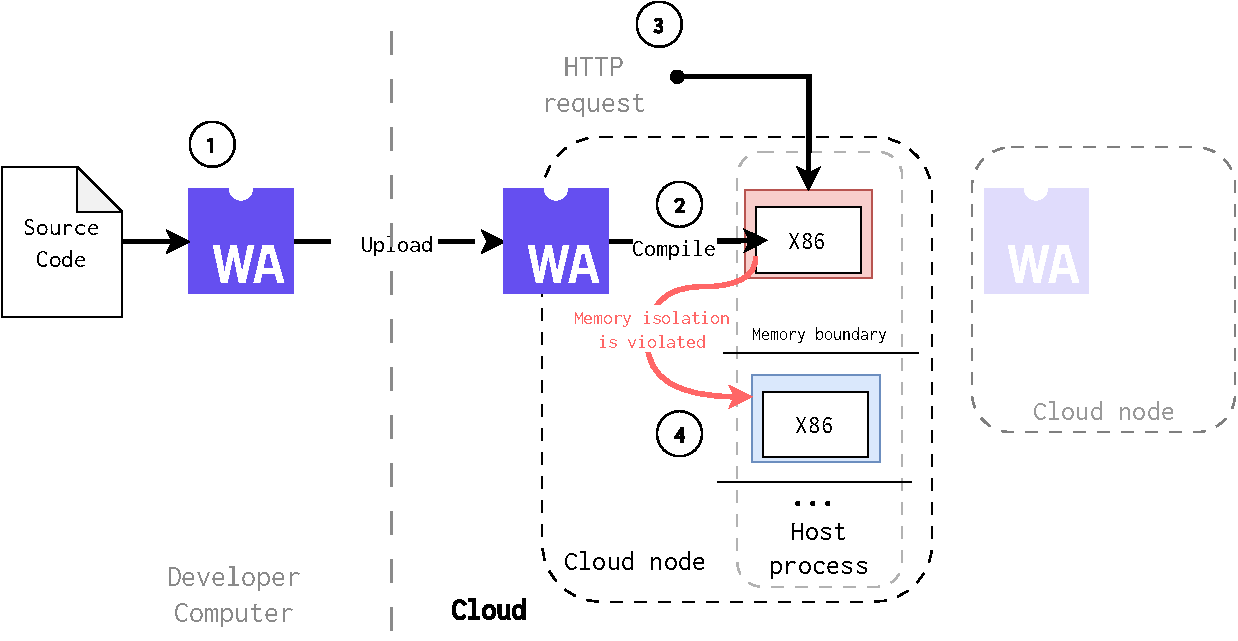
\includegraphics[width=0.8\linewidth]{figures/edge.pdf}
    \caption{\Wasm binaries on FaaS platforms.}
    \label{fig:edge_model}
\end{figure}

The fundamental advantage of using \Wasm in FaaS platforms lies in its ability to encapsulate thousands of client \Wasm binaries within a singular host process.
A developer could compile its source code into a \Wasm program suitable for the cloud platform and then submit it (\step{1} in \autoref{fig:edge_model}).
This host process is then disseminated across a network of servers and data centers (\step{2} in \autoref{fig:edge_model}). 
These platforms convert \Wasm programs into native code, which is subsequently executed in a sandboxed environment. 
Host processes can then instantiate new \Wasm sandboxes for each client function, executing them in response to specific user requests with nanosecond-level latency (\step{3} in \autoref{fig:edge_model}). 
This architecture inherently isolates \Wasm binary executions from each other as well as from the host process, enhancing security.

However, while \Wasm is engineered with a strong on security and isolation, it is not entirely immune to vulnerabilities such as Spectre attacks \cite{Spectre,Narayan2021Swivel} (\step{4} in \autoref{fig:edge_model}). 
In the sections that follow, we explore how software diversification techniques can be employed to fortify \Wasm binaries against such attacks. 
Specifically, we discuss the concept of Defensive Software Diversification, aimed at enhancing the security of \Wasm binaries by generating a multitude of diverse and unique \Wasm variants that can be randomized during deployment.

\msubsection{Threat model: speculative side-channel attacks}

To illustrate the threat model concerning \Wasm programs in FaaS platforms, consider the following scenarios. 
Developers, including potentially malicious actors, have the ability to submit any \Wasm binary to the FaaS platform. 
A malicious actor could upload a \Wasm binary that, once compiled to native code, employs Spectre attacks to either leak sensitive information from the host process or violate Control Flow Integrity (CFI).
Furthermore, even if a submitted \Wasm binary is not intentionally malicious, it may still be vulnerable to Spectre attacks. 
For instance, a malicious actor could exploit this vulnerability by executing the susceptible binary through the FaaS service. 

Spectre attacks exploit hardware-based prediction mechanisms to trigger mispredictions, leading to the speculative execution of specific instruction sequences, commonly referred to as \emph{gadgets} \cite{gadgets}.
These gadgets would not be part of the standard, sequential execution flow. 
By taking advantage of this speculative execution, an attacker can potentially access sensitive information stored in the memory allocated to other \Wasm instance(including itself) or even the host process itself. 
This poses a significant risk, compromising both the security and integrity of the overall system.

Narayan and colleagues \cite{Narayan2021Swivel} have categorized potential Spectre attacks on \wasm binaries into three distinct types, each corresponding to a specific hardware predictor being exploited and a particular FaaS scenario: Branch Target Buffer Attacks,  Return Stack Buffer Attacks, and Pattern History Table Attacks defined as follows:

\begin{enumerate}
    \item The Spectre Branch Target Buffer (btb) attack exploits the branch target buffer by predicting the target of an indirect jump, thereby rerouting speculative control flow to an arbitrary target.
    \item  The Spectre Return Stack Buffer (rsb) attack exploits the return stack buffer that stores the locations of recently executed call instructions to predict the target of \texttt{ret} instructions.
    \item The Spectre Pattern History Table (pht) takes advantage of the pattern history table to anticipate the direction of a conditional branch during the ongoing evaluation of a condition.
\end{enumerate}


%\lipsum[1]

%\lipsum[1]

\msubsection{Methodology}

Our goal is to empirically validate that Software Diversification can effectively mitigate the risks associated with Spectre attacks in \Wasm binaries. 
The green-highlighted section in \autoref{fig:defense_model} illustrates how Software Diversification can be integrated into the FaaS platform workflow. 
The core idea is to generate unique and diverse \Wasm variants that can be randomized at the time of deployment. 
For this use case, we employ WASM-MUTATE as our tool for Software Diversification.

To empirically demonstrate that Software Diversification can indeed mitigate Spectre vulnerabilities, we utilize the \Wasm binaries proposed by Narayan and colleagues in their work on Swivel \cite{Swivel}. 
Swivel is a compiler-based strategy designed to counteract Spectre attacks on \Wasm binaries by linearizing their control flow during machine code compilation. 
Our approach differs from theirs in that it is binary-based, compiler-agnostic, and platform-agnostic; we do not propose altering the deployment or toolchain of FaaS platforms. 
Although our experiments are conducted prior to submitting the \Wasm binary to the FaaS platform, we argue that \Wasm binary diversification could be implemented at any stage of the FaaS workflow.
The same argument holds by using any other diversification technique included in this dissertation (see \autoref{tech}).


\begin{figure}[h]
    \centering
    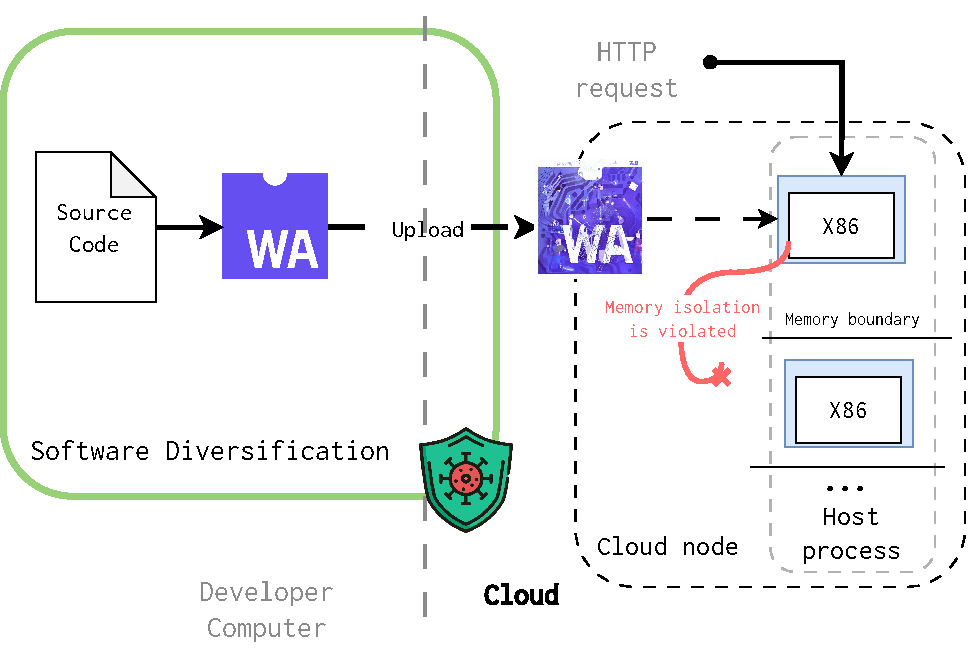
\includegraphics[width=0.75\linewidth]{figures/edge_protected.pdf}
    \caption{Diversifying \Wasm binaries to mitigate Spectre attacks in FaaS platforms.}
    \label{fig:defense_model}
\end{figure}

\begin{table}
    \centering
    \begin{tabular}{l | l  }
        \hline
         Program &  Attack  \\
        \hline \hline
        btb\_breakout & Spectre branch target buffer (btb)  \\
        \hline
         btb\_leakage & Spectre branch target buffer(btb)  \\
        \hline
         ret2spec &  Spectre Return Stack Buffer (rsb)  \\
        \hline
        pht &  Spectre Pattern History Table (pht)  \\

%\end{adjustbox}
    \end{tabular}
    \caption{}
    \label{programs}
\end{table}

To measure the efficacy of WASM-MUTATE in mitigating Spectre, we diversify four \Wasm binaries proposed in the Swivel study. 
The details of these programs and the specific attacks we examine are available in \cite{programs}. 
For each of these four binaries, we generate up to 1000 random stacked transformations using 100 distinct seeds, resulting in a total of 100,000 variants for each original binary. 
At every 100th stacked transformation for each binary and seed, we assess the impact of diversification on the Spectre attacks by measuring the attack bandwidth for data exfiltration. 
This metric not only captures the success or failure of the attacks but also quantifies the extent to which data exfiltration is hindered. 
For example, a variant that still leaks data but does so at an impractically slow rate would be considered hardened against the attack.

\begin{definition}{Attack bandwidth:}\label{metric:ber}
    Given data $D=\{b_0, b1, ..., b_C\}$ being exfiltrated in time $T$ and $K = {k_1, k_2, ..., k_N}$ the collection of correct data bytes, the bandwidth metric is defined as:
    $$
        \frac{|b_i\text{ such that } b_i \in K|}{T}
    $$
\end{definition}


\msubsection{Results}

- Diminshing of BER
- Rockiki paper on portable side channel in browsers.



\todo{TBD discuss deoptimization}
% \subsection{Deoptimization}

\begin{tcolorbox}[title=Contribution paper,boxrule=1pt,arc=.2em,boxsep=1.0mm]
    The case discussed in this section is fully detailed in Cabrera-Arteaga \etal "WASM-MUTATE: Fast and Effective Binary Diversification for WebAssembly"
    \emph{Under review}
    \url{https://arxiv.org/pdf/2309.07638.pdf}. 
\end{tcolorbox}



